% 波的能量
% 能量|平面波|能量密度|势能

\pentry{一维波动方程\upref{WEq1D},二项式定理(非整数幂)\upref{BiNorR}}

\subsection{波的能量}
当机械波传播到介质中的某处时,该处原来不动的质点开始振动,因而具有\textbf{动能},同时该处的介质也将产生形变,因而也具有\textbf{势能}.

波动传播时,介质由近及远地振动着,由此可见,能量是向外传播的.这是波动的重要特征.

\begin{figure}[ht]
\centering
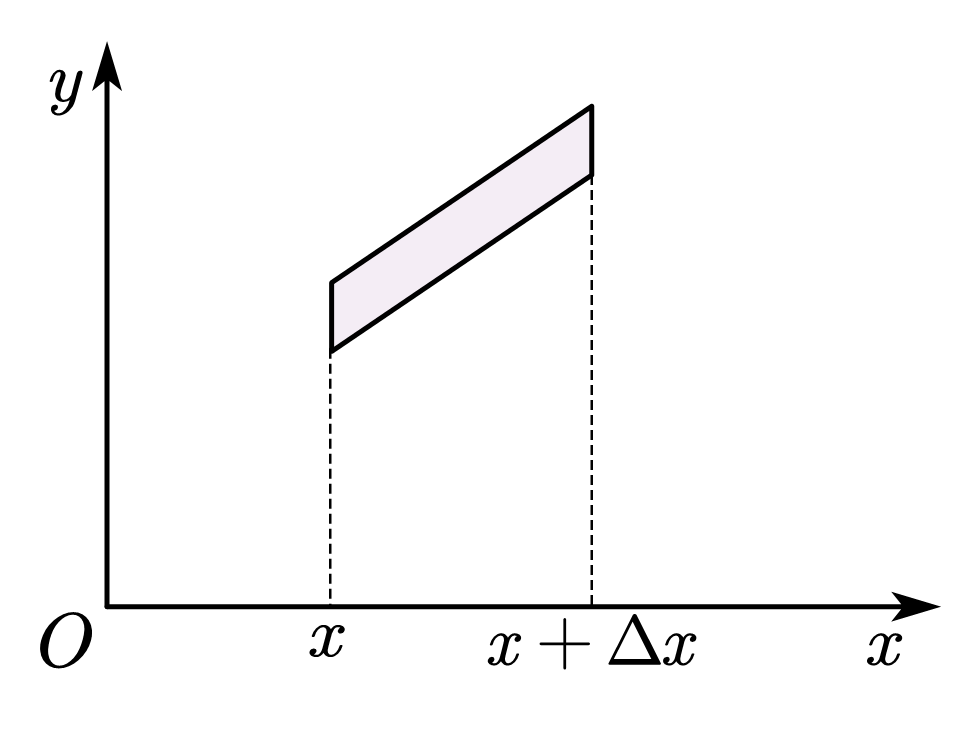
\includegraphics[width=5cm]{./figures/WaEner_1.png}
\caption{一小段线元} \label{WaEner_fig1}
\end{figure}

如\autoref{WaEner_fig1}所示,在弦线上在$x$处取线元$\Delta x$,设弦线的线密度(单位长度的质量)为$\rho_l$,其质量为$\rho_l\Delta x$.
当弦线中有平面简谐波传播时,设波函数为
\begin{equation}
y=A \cos \left[\omega\left(t-\frac{x}{u}\right)+\phi_{0}\right]
\end{equation}
线元的动能为
\begin{equation}
\Delta E_{\mathrm{k}}=\frac{1}{2} \rho_{l} \Delta x\left(\frac{\partial y}{\partial t}\right)^{2}
\end{equation}
弦线上有张力作用,线元由原长$\Delta x$变为$\Delta l$,也就是说伸长了$\Delta l-\Delta x$.这是在张力的作用下伸长的,即它的弹性势能应等于弦张力$F$在线元伸长过程中做的功,也就是
\begin{equation}
\Delta E_{\mathrm{p}}=F(\Delta l-\Delta x)
\end{equation}
在$\Delta x$很小时
\begin{equation}
\begin{aligned} \Delta l &=\sqrt{(\Delta x)^{2}+(\Delta y)^{2}}=\Delta x\left[1+\left(\frac{\Delta y}{\Delta x}\right)^{2}\right]^{1 / 2} \\ & \approx \Delta x\left[1+\left(\frac{\partial y}{\partial x}\right)^{2}\right]^{1 / 2} \approx \Delta x\left[1+\frac{1}{2}\left(\frac{\partial y}{\partial x}\right)^{2}\right] \end{aligned}
\end{equation}
此处的最后一个约等号运用了广义二项式定理(\autoref{BiNorR_eq2}\upref{BiNorR}).
因此
\begin{equation}
\Delta E_{\mathrm{p}}=\frac{1}{2} F\left(\frac{\partial y}{\partial x}\right)^{2} \Delta x
\end{equation}
所以,线元的总机械能
\begin{equation}
\Delta E=\Delta E_{\mathrm{k}}+\Delta E_{\mathrm{p}}=\frac{1}{2} \rho_{l}\left(\frac{\partial y}{\partial t}\right)^{2} \Delta x+\frac{1}{2} F\left(\frac{\partial y}{\partial x}\right)^{2} \Delta x
\end{equation}
对于平面简谐波有
\begin{equation}
\Delta E_{\mathrm{k}}=\frac{1}{2} \rho_{l} \Delta x\left(\frac{\partial y}{\partial t}\right)^{2}=\frac{1}{2} \rho_{l} \Delta x \omega^{2} A^{2} \sin ^{2}\left[\omega\left(t-\frac{x}{u}\right)+\phi_{0}\right]
\end{equation}
\begin{equation}
\Delta E_{\mathrm{p}}=\frac{1}{2} F \Delta x\left(\frac{\partial y}{\partial x}\right)^{2}=\frac{1}{2} F \Delta x \frac{1}{u^{2}} \omega^{2} A^{2} \sin ^{2}\left[\omega\left(t-\frac{x}{u}\right)+\phi_{0}\right]
\end{equation}
由于$u=\sqrt{\dfrac{F}{\rho_{l}}}$,所以有
\begin{equation}
\Delta E_{\mathrm{p}}=\frac{1}{2} \rho_{l} \Delta x \omega^{2} A^{2} \sin ^{2}\left[\omega\left(t-\frac{x}{u}\right)+\phi_{0}\right]
\end{equation}
即
\begin{equation}
\Delta E_{\mathrm{p}}=\Delta E_{\mathrm{k}}
\end{equation}
而总机械能为
\begin{equation}
\Delta E=\Delta x \rho_{l} \omega^{2} A^{2} \sin ^{2}\left[\omega\left(t-\frac{x}{u}\right)+\phi_{0}\right]
\end{equation}

\subsection{能量密度}

为了更精确地描述波在介质中的分布情况,引入能量密度的概念.

介质中单位体积的波动能量,称为\textbf{波的能量密度},用$w$表示.设弦线的横截面积为$S$,其体密度为$\rho$,它与线密度$\rho_l$的关系为$\rho_l=\rho S$.则能量密度
\begin{equation}
w=\frac{\Delta E}{S \Delta x}=\rho \omega^{2} A^{2} \sin ^{2}\left[\omega\left(t-\frac{x}{u}\right)+\phi_{0}\right]
\end{equation}
波的能量密度是随时间而变化的,通常取其在一个周期内的平均值,用$\overline w$表示,称为\textbf{平均能量密度}.因为正弦函数的平方在一个周期内的平均值为$\dfrac 12$,即
\begin{equation}
\frac{1}{T} \int_{0}^{T} \sin ^{2} \omega t \mathrm{d} t=\frac{1}{2}
\end{equation}
所以能量密度在一个周期内的平均值为
\begin{equation}
\overline{w}=\frac{1}{2} \rho A^{2} \omega^{2}
\end{equation}

由上式可见,机械波的能量与振幅的平方、频率的平方都成正比.